\section{Unmanned aerial vehicle}
\label{sec:unmanned-aerial-vehicle}
%
%
An unmanned aerial vehicle UAV (commonly known as a drone) is an aircraft 
without a human pilot on board and a type of unmanned vehicle. 
UAVs are a component of an unmanned aircraft system (UAS); which include a UAV,
a ground-based controller, and a system of communications between the two.\\
The flight of UAVs may operate with various degrees of autonomy: either under
remote control by a human operator or autonomously by on-board computers.
Compared to crewed aircraft, UAVs were originally used for missions too
dangerous for humans.\cite{budiansky2005air}\\
While they originated mostly in military applications, their use is rapidly
expanding to commercial, scientific, recreational, agricultural, policing and
surveillance, product deliveries, aerial photography, infrastructure
inspections, and drone racing.\cite{wiki:uav}
%
%
\begin{figure}[htb]
    \centering
    \subfloat[][\emph{Northrop Grumman Bat carrying EO/IR and SAR sensors, laser range finders, laser designators, Infra-Red cameras}.]{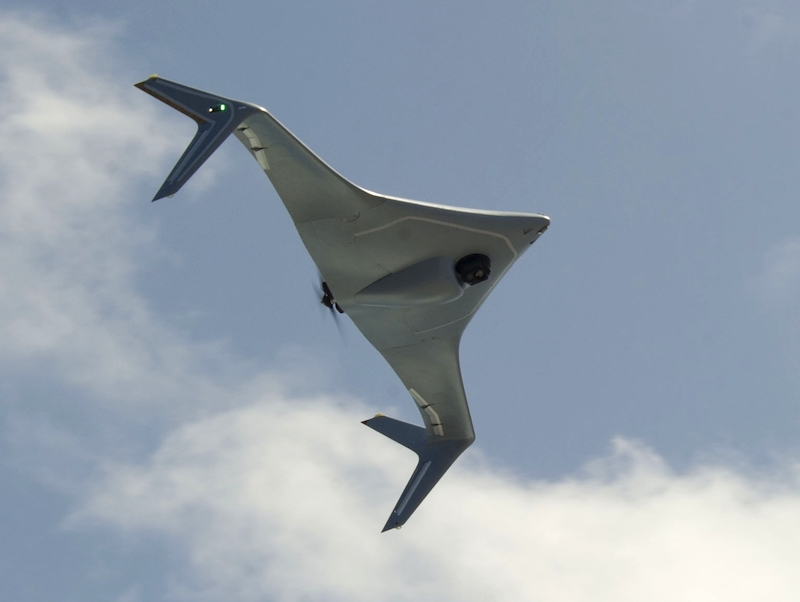
\includegraphics[width=.40\textwidth]{Northrop_Grumman_Bat_UAV_in_flight_in_June_2014.JPG}} \\
    \subfloat[][\emph{A DeltaQuad VTOL fixed wing surveillance UAV}.]{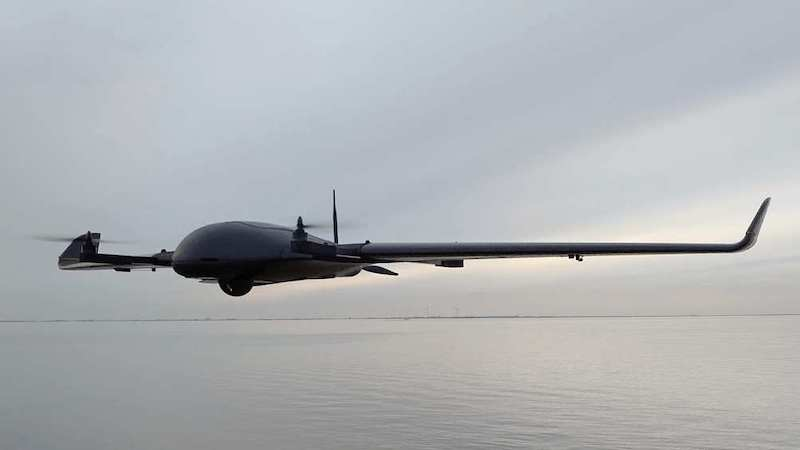
\includegraphics[width=.40\textwidth]{DeltaQuad_VTOL_surveillance_UAV.jpg}}
    \captionsource{UAVs used in various operations.}{
    \href{https://en.wikipedia.org/wiki/Unmanned_aerial_vehicle}{Wikipedia}}
    \label{fig:uavs-image}
\end{figure}
%
%
\subsection{UAV components}
\label{ssec:components}
%
Crewed and un-crewed aircraft of the same type generally have recognizably
similar physical components. One of the differences is the absence of the
cockpit and environmental control system or life support systems. Some UAVs
carry payloads such as a camera or other kinds sensors smaller and lightweight.
Small UAVs have assumed a characteristic quad-copter design particular
recognizable, although other scheme are realizable.
With the continuous development in the introduction of new parts or revisited 
ones the process of miniaturized require less-power propulsion and increase
battery runtime.\\
Control systems for UAVs are different for remote human control, a camera and
video link almost always replace the cockpit windows; radio-transmitted digital
commands replace physical cockpit controls. Autopilot software is used on both
crewed and uncrewed aircraft, with varying feature sets.\cite{wiki:uav}
%
%
\begin{figure}[htb]
    \centering
    \subfloat[][\emph{typical quadcopter design}.\label{subfig:quadcopter-design}]{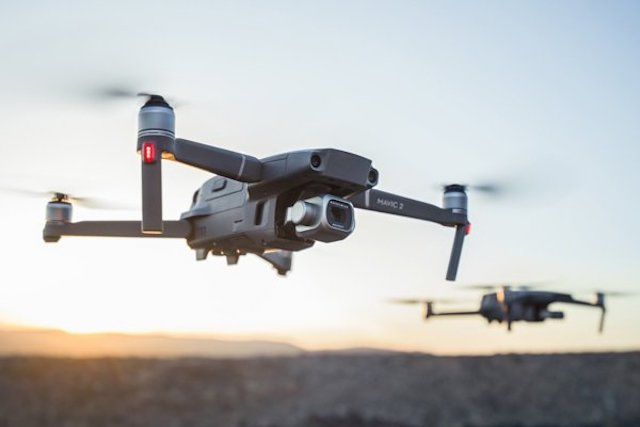
\includegraphics[width=.50\textwidth]{dji_mavic_2-1.jpg}} \quad
    \subfloat[][\emph{multirotor drone design}.\label{subfig:multicopter}]{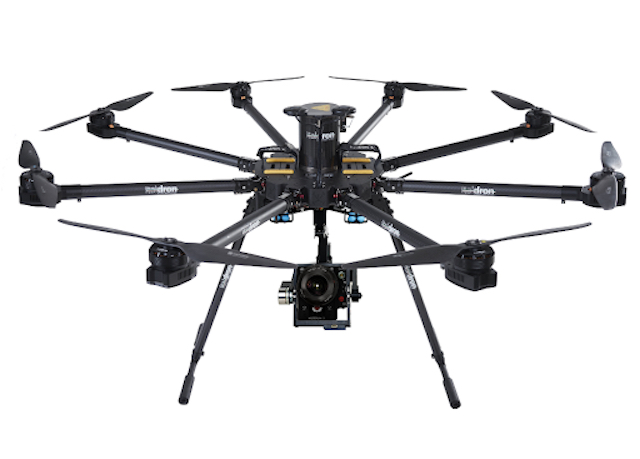
\includegraphics[width=.50\textwidth]{unnamed.jpg}}
    \captionsource{Example of design choices in the realization of UAVs shape}{
    \href{https://www.dji-store.it/guida-acquisto-migliori-droni-dji-per-riprese-aeree/}{DJI}; 
    \href{http://www.italdron.com/it/droni-professionali-e-accessori/droni-professionali/bigone-8hse-pro}{Italdron}}
    \label{fig:uav-design}
\end{figure}
%
%
\paragraph{Body} UAVs assume different configuration based on requirement of
task they perform for example aerial video shooting, surveys, territorial
control and many more.
Thus they are normally equipped with 4, 6, or 8 motor called quadcopter,
exacopter or octocopter.
The mainly difference that exist between different configuration is the payload
capacity that it can carry in flight.
%
\paragraph{Power supply}
Small UAVs mostly use lithium-polymer batteries (Li-Po), while larger vehicles
rely on conventional airplane engines. Scale or size of aircraft is not the
defining or limiting characteristic of energy supply for a UAV. 
Battery elimination circuitry (BEC) is used to centralize power distribution and
often harbors a microcontroller unit (MCU). Costlier switching BECs diminish
heating on the platform.\cite{wiki:uav}
%
\paragraph{Hardware}
systems mounted on the drone have undergone an evolution in step
with the advancement of the IT sector, so much so that the analog controls have
been gradually replaced by microcontrollers up to System On Chip (SoC) with
single board cmaputer such as the Raspberry. In addition, UAVs are equipped with
flight controllers, flight controller boards and autopilots.
%
\paragraph{Sensors and Actuators}
Drone control is allowed through the cooperation of proprioceptive and
exteroceptive sensors that send their information to the central processing
unit.
The data coming from the platform measures accelerations and angular speeds
through accelerometers and gyroscopes that process and transmit the attitude
data such as orientation and position.
The GPS allows the spatial location of the aircraft on a map and to control the
route with respect to a planned trajectory. The altimeter allows you to
continuously record changes in altitude. The magnetometer is a device that
allows you to define the magnetic field vector at the point where you measure
with the drone and then obtain the orientation with respect to the North.
Knowledge and control of these measures allows the central system to allow
control of the actuators. Other more less common sensors may be present to
perform the most varied tasks.
%
\paragraph{Communications}
Most UAVs use a radio for remote control and exchange of video and other data.
The connections depending on the use cases and needs can be narrowband and
broadband. Generally, the sending and receiving of the commands is carried out
by means of a radio connection from the ground, especially for remote piloting.\\
Other connections that exploit protocols such as TCP/IP are used for sending
multimedia data such as filming areas and are transmitted to mobile devices such
as smartphones, tablets and so on.
Other types of connections can be used depending on the sector of use, in fact
for the military sector these may differ to ensure greater safety and
robustness.\\ 
More and more UAVs are implementing the MAVlink protocol for the
transport of data of control and control between piloting on the ground and
aircraft.
%
%
\subsection{Autonomy}
\label{ssec:autonomy}
%
UAVs have various levels of autonomy, that is, they are not completely
autonomous and do not require continuous intervention by the remote operator.
They have algorithms of return to the house which can be performed with a certain
level of autonomy. 
Up to high levels of autonomy which allow more complex operations. 
Autonomy derives from the awareness of the situation in which the drone is
located. 
The knowledge derives from the data acquired by the sensors mounted on board the
drone. 
The use of sensor fusion to integrate the information collected allows to limit
the error committed and to increase the precision and accuracy of the
information obtained. 
UAV's degrees of autonomy are often implemented by UAV manufacturers often build
in specific autonomous operations, such as:
\begin{itemize}
	\item Self-level: attitude stabilization on the pitch and roll axes.
	\item Altitude hold: The aircraft maintains its altitude using barometric or ground sensors.
	\item Hover/position hold: Keep level pitch and roll, stable yaw heading and altitude while maintaining position using GNSS or inertal sensors.
	\item Headless mode: Pitch control relative to the position of the pilot rather than relative to the vehicle's axes.
	\item Care-free: automatic roll and yaw control while moving horizontally.
	\item Take-off and landing (using a variety of aircraft or ground-based sensors and systems; see also:Autoland)
	\item Failsafe: automatic landing or return-to-home upon loss of control signal.
	\item Return-to-home: Fly back to the point of takeoff (often gaining altitude first to avoid possible intervening obstructions such as trees or buildings).
	\item Follow-me: Maintain relative position to a moving pilot or other object using GNSS, image recognition or homing beacon.
	\item GPS waypoint navigation: Using GNSS to navigate to an intermediate location on a travel path.
	\item Orbit around an object: Similar to Follow-me but continuously circle a target.
	\item Pre-programmed aerobatics (such as rolls and loops).\cite{wiki:uav}
\end{itemize}
%
%
\begin{figure}[htb]
	\centering
    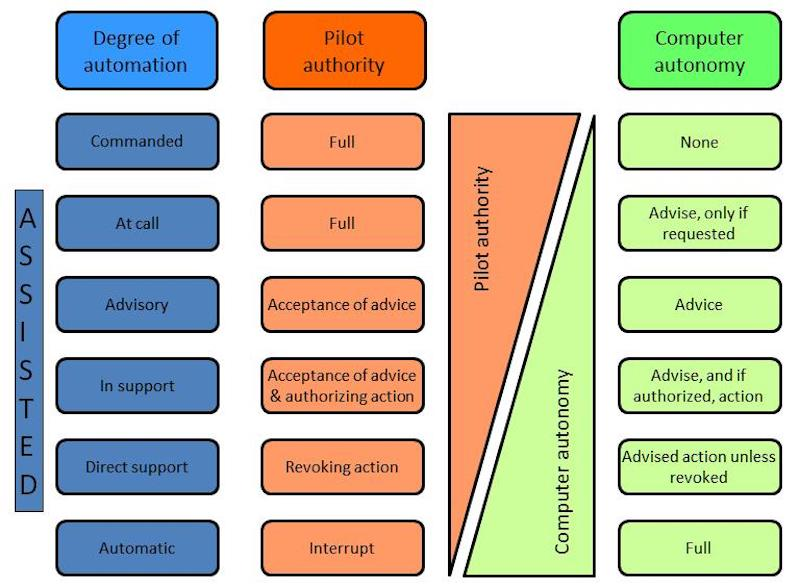
\includegraphics[width=0.50\textwidth]{Degrees_of_autonomy.jpg}
    \captionsource{UAV's degrees of autonomy.}{\href{https://en.wikipedia.org/wiki/Unmanned_aerial_vehicle}{Wikipedia}}
    \label{fig:uav-autonomy}
\end{figure}
%